\documentclass[../CSC_5RO07_TA.tex]{subfiles}

\begin{document}
\section{Q2: Multicoeur 3 coeurs : 1 ARM et 2 MicroBlaze}

\subsection{Traitement d'image : filtre Sobel}

Pour tester le système multicœur, il a été décidé de l'utiliser dans une tâche de traitement d'image, car en raison de sa nature, où il est nécessaire de faire plusieurs multiplications tout au long du processus, cette option semble correcte pour tester autant que possible les possibilités et les possibilités. portée du système. 

\vspace{1em} 

Sachant cela, il a été décidé d'utiliser le filtre Sobel pour détecter les bords de l'image ; Ceci est basé sur l’identification de changements brusques d’intensité lumineuse dans une image. Cette méthode utilise des masques (ou noyaux) qui permettent de calculer les gradients d'intensité dans deux directions principales : horizontale ($G_x$) et verticale ($G_y$) (Figure \ref{fig:1}).

\begin{figure}[H]
    \centering
    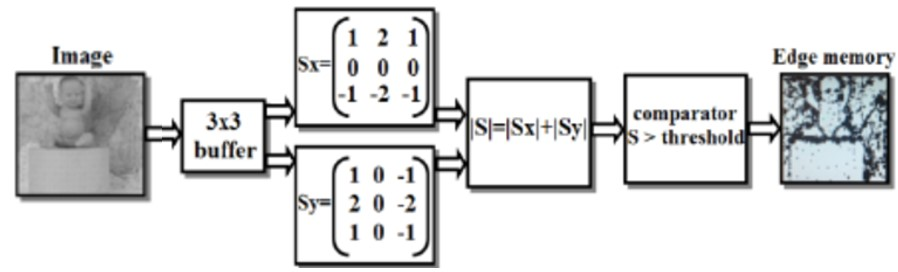
\includegraphics[width=0.7\columnwidth]{./images/FiltreSobel.jpg}
    \caption{Schéma explicatif du flux de travail du système.}
    \label{fig:1}
\end{figure}

Pour appliquer le filtre Sobel, l'image originale doit être en niveaux de gris, puisque les calculs de dégradé sont effectués sur des valeurs d'intensité. Les masques de filtre sont de petites matrices qui mettent en évidence le taux de changement de l'intensité des pixels dans chaque direction. Le masque horizontal ($G_x$) est utilisé pour détecter les bords verticaux, tandis que le masque vertical ($G_y$) met en évidence les bords horizontaux. Ces masques convoluent avec l'image originale, ce qui signifie qu'ils se déplacent pixel par pixel à travers l'image, multipliant leurs valeurs par celles des pixels correspondants du voisinage, puis additionnant les résultats. Il en résulte une image qui met en évidence des zones de changement brusque d'intensité dans la direction correspondant à chaque masque. 

\vspace{1em} 

Après avoir appliqué les deux masques, les résultats $G_x$ et $G_y$ sont combinés pour calculer l'ampleur du dégradé total à chaque pixel. L'ampleur du gradient, donnée par la formule $G = \sqrt{G_x^2 + G_y^2}$, représente l'intensité des bords. Plus la valeur de pente est élevée, plus le bord est raide à cet endroit. Cela génère une nouvelle image en niveaux de gris dans laquelle les bords sont clairement visibles. 

\vspace{1em} 

Le filtre Sobel est populaire en raison de sa simplicité et de son efficacité. Ce filtre est un outil essentiel en vision par ordinateur, utilisé dans des tâches telles que la détection de contours, la détection d'objets et l'analyse d'images médicales, entre autres.

\subsection{Flux de travail}

Le flux de traitement est expliqué ci-dessous, qui implique la transmission, le partitionnement, le traitement parallèle et la reconstruction d'une image grâce à la collaboration entre un ordinateur, un ARM 9 et deux processeurs MicroBlaze. Chaque étape du processus est détaillée ci-dessous et est visible dans la figure \ref{fig:2} :

\begin{figure}[H]
    \centering
    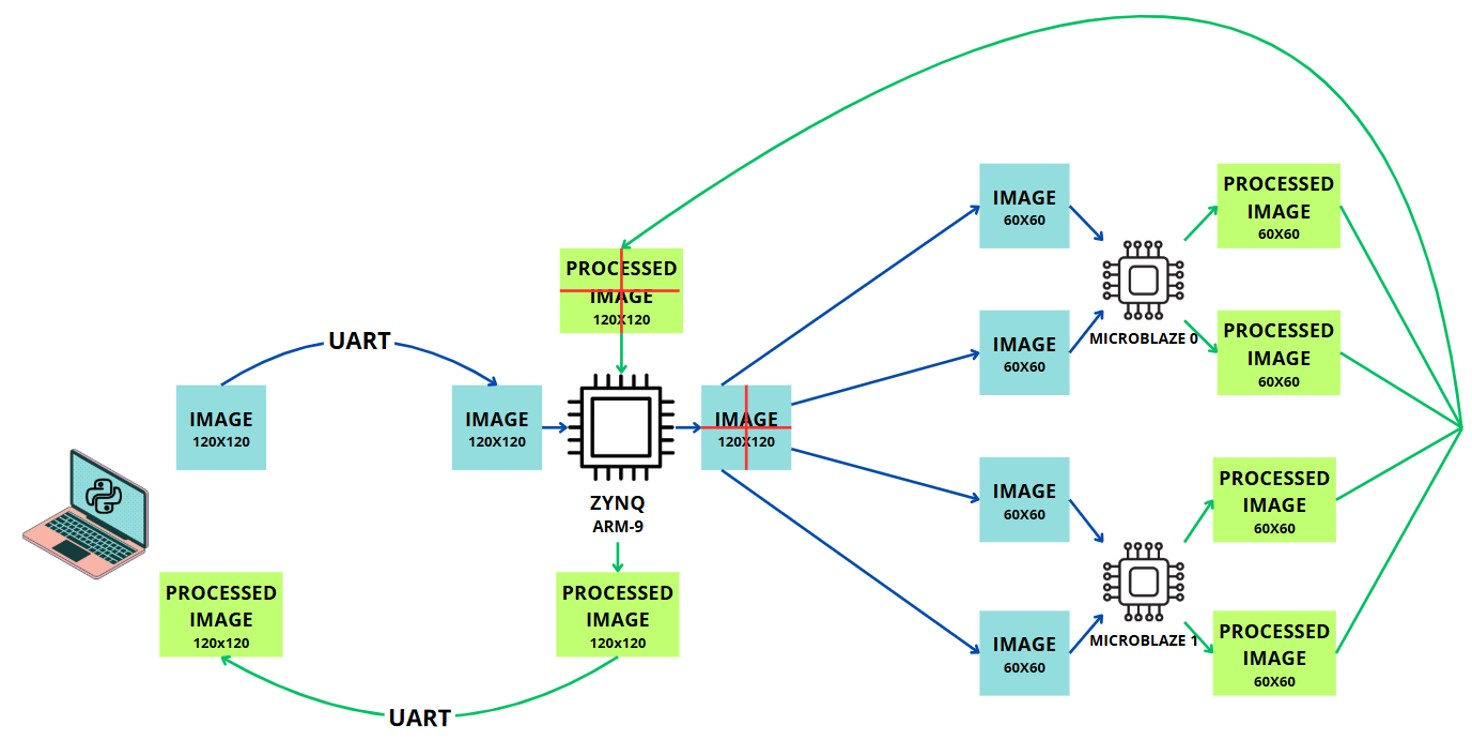
\includegraphics[width=0.8\columnwidth]{./images/DiagramaBloques3x3.jpg}
    \caption{Schéma explicatif du flux de travail du système.}
    \label{fig:2}
\end{figure}

\begin{enumerate}

\item L'ordinateur fait office de source de données initiale, envoyant une image à l'ARM 9 via l'interface UART.

\item Dès réception de l'image complète, l'ARM 9 la divise en quatre sous-images de dimensions égales. Cette partition est destinée à répartir la charge de traitement uniformément entre les processeurs MicroBlaze disponibles. Chaque sous-image est mappée sur une région spécifique de mémoire partagée entre l'ARM 9 et le MicroBlaze.

\item L'ARM 9 attribue deux sous-images à chaque processeur MicroBlaze :
\begin{itemize}
    \item Le **MicroBlaze 0** reçoit deux sous-images correspondant à la moitié supérieure de l'image (les deux premiers quarts).
    \item Le **MicroBlaze 1** s'occupe des deux sous-images restantes, correspondant à la moitié inférieure de l'image (les deux derniers quarts).
 Cette répartition égale permet aux deux processeurs de travailler simultanément sur des tâches de traitement spécifiques.
\end{itemize}

\item Chaque MicroBlaze effectue des opérations pour utiliser le filtre Sobel sur les sous-images attribuées. Ces opérations consistent en plusieurs multiplications matricielles, additions et calculs de racine. Le résultat de ce traitement est deux sous-images traitées par chaque MicroBlaze.

\item Une fois le traitement terminé, les MicroBlazes écrivent les sous-images traitées dans les régions désignées de la mémoire partagée. Cette mémoire fait office de moyen d'échange de données entre les processeurs et l'ARM 9.

\item L'ARM 9 récupère les sous-images traitées de la mémoire partagée et les combine pour reconstruire l'image complète de 120 x 120 pixels. Cette étape garantit que les quatre sous-images sont réassemblées à leur emplacement d'origine pour former une représentation cohérente de l'image traitée.

\item Enfin, l'ARM 9 transmet l'image traitée à l'ordinateur via l'interface UART.

\end{enumerate}

\subsection{Diagramme de blocs}

\begin{figure}[H]
    \centering
    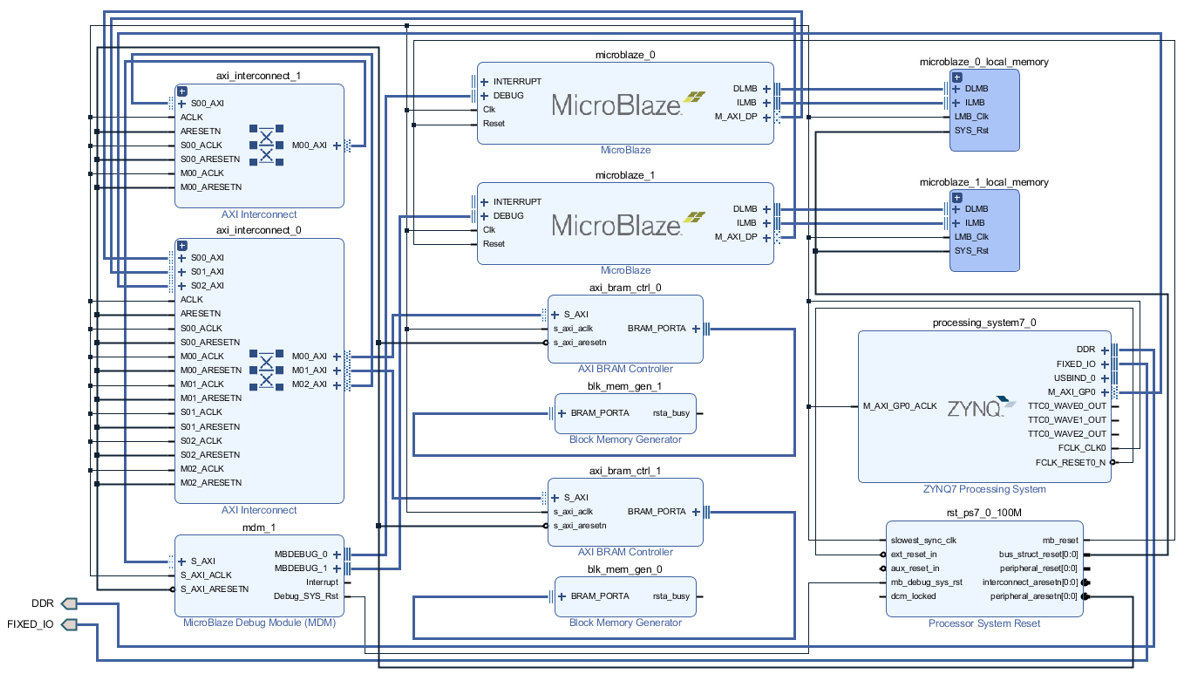
\includegraphics[width=\textwidth]{img1.png}
    \caption{Diagramme de blocs du système multicoeur 1 ARM et 2 Microblaze}
    \label{fig:3}
\end{figure}

Le système présenté combine un processeur \textbf{ZYNQ7 Processing System} et deux processeurs \textbf{MicroBlaze}, conçu pour le traitement d'images. Le \textbf{ZYNQ7}, avec ses deux cœurs ARM Cortex-A9, agit comme le noyau principal, gérant les tâches générales, la communication avec les périphériques et le transfert de données vers les mémoires DDR et les blocs logiques programmables. Sa puissance en fait un choix idéal pour manipuler de grands volumes de données, comme les images, tout en coordonnant les autres blocs.

\vspace{1em} 

Les processeurs \textbf{MicroBlaze} apportent de la flexibilité au système et sont spécialement configurés pour effectuer la détection des contours dans les images. Ils fonctionnent en parallèle, se partageant les calculs des matrices nécessaires au traitement. Cette approche parallèle optimise les performances et accélère considérablement les opérations. La capacité des MicroBlaze à s'adapter à des tâches spécifiques et à opérer de manière autonome en fait des éléments essentiels de ce design.

\vspace{1em} 

Pour relier tous les composants, les \textbf{AXI Interconnects} agissent comme des autoroutes, organisant le trafic des données entre les processeurs, les mémoires et les périphériques. Cela est crucial, car le traitement d’images exige des transferts rapides et efficaces de grandes quantités de données. De plus, le \textbf{MicroBlaze Debug Module} permet de vérifier que les processeurs MicroBlaze fonctionnent correctement, facilitant le débogage pendant le développement et garantissant que les tâches de traitement spécifiques sont réalisées sans erreur.

\vspace{1em} 

Le module \textbf{Processor System Reset} garantit que le système démarre de manière ordonnée et synchronisée, évitant tout dysfonctionnement au démarrage et assurant la stabilité globale du design. Chaque MicroBlaze dispose de sa propre mémoire locale (\textit{DLMB} et \textit{ILMB}), ce qui leur permet de fonctionner de façon indépendante et rapide, en stockant les données et les instructions nécessaires au traitement en temps réel.

\vspace{1em} 

Par ailleurs, les \textbf{BRAM (Block RAM)}, gérées par les \textbf{AXI BRAM Controllers} et les \textbf{Block Memory Generators}, jouent un rôle fondamental en tant que buffers rapides. Elles permettent de stocker temporairement des fragments d’images ou des résultats intermédiaires pendant que les MicroBlaze effectuent les calculs nécessaires à la détection des contours, réduisant la latence et augmentant l'efficacité du système.

\vspace{1em} 

Dans l’ensemble, ce design exploite la puissance du ZYNQ pour les tâches générales, la capacité des MicroBlaze pour un traitement dédié, les BRAM pour un stockage rapide, et les interconnects pour un flux de données ordonné. C’est une solution robuste et évolutive, idéale pour le traitement d’images, où la rapidité et la capacité à gérer de grands volumes de données sont essentielles.

\subsection{Mémoires}
Le système implémente une structure de mémoire hiérarchique conçue pour optimiser l'interaction entre deux processeurs MicroBlaze et un système ZYNQ basé sur un ARM Cortex-A9. Ce schéma organise et segmente la mémoire pour diviser efficacement la charge de travail entre différents éléments, facilitant ainsi le traitement parallèle et la gestion des ressources.
\vspace{1em} 

Le système utilise deux principaux types de mémoire :
Chaque MicroBlaze a accès à deux BRAM locales :
\begin{itemize}
    \item DLMB (Data Local Memory Bus) : Pour stocker et accéder aux données.
    \item ILMB (Instruction Local Memory Bus) : Exclusif pour les instructions du programme.
 \end{itemize}
 Ces mémoires sont conçues pour un accès rapide et sont directement associées à chaque MicroBlaze, améliorant ainsi l'efficacité des opérations locales.

\vspace{1em} 
DDR (Dynamic RAM) : la mémoire DDR est gérée par l'ARM 9 et est utilisée pour stocker les images, à la fois en entrée et en sortie, et pour la coordination entre les éléments du système. A partir de cette mémoire, sont définis deux blocs qui serviront au transfert de données entre l'ARM 9 et les deux Microblaze. Cette application est réalisée en parallélisant complètement l'accès à la mémoire du Microblaze, ainsi les données utilisées par le premier Microblaze se trouvent dans un bloc mémoire spécifique \textbf{(0x40000000 - 0x40007fff}) et les données du deuxième Microblaze dans un autre bloc \textbf{(0x42000000 - 0x42007fff)}. Cela garantit que pendant le traitement de l'image, il n'y a pas de conflits d'entrée en mémoire, améliorant ainsi le temps d'exécution et évitant les plantages. Pour cette raison, il a été défini que les masques de convolution utilisés dans le traitement, ($G_x$) et ($G_y$), sont stockés de manière redondante dans les BRAM de chaque MicroBlaze.

\vspace{1em} 

Toutes les mémoires locales (DLMB et ILMB) et les blocs DDR ont été configurés avec une taille de 32 Ko. Cette valeur a été sélectionnée en fonction de la taille des images à traiter, garantissant suffisamment d'espace pour stocker les données nécessaires sans gaspiller de ressources. Ces valeurs sont visibles sur la figure \ref{fig:4}.

\begin{figure}[H]
    \centering
    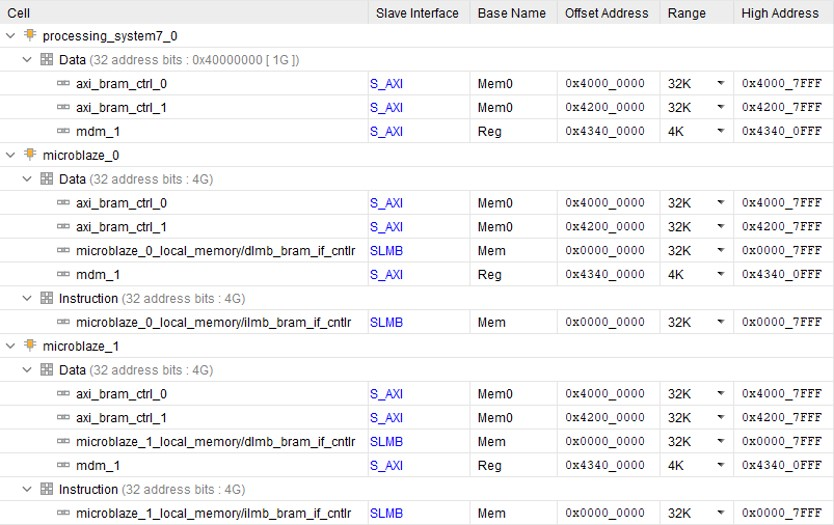
\includegraphics[width=1.0\columnwidth]{./images/Memoria.jpg}
    \caption{Répartition de la mémoire.}
    \label{fig:4}
\end{figure}

Le flux de traitement de la mémoire est :

\begin{enumerate}
    \item Les images d'entrée sont initialement stockées dans des régions spécifiques du DDR.
    \item L'ARM 9 distribue les sous-images aux BRAM correspondantes du MicroBlaze.
    \item Chaque MicroBlaze traite les sous-images attribuées en utilisant ses mémoires locales (DLMB et ILMB) et les masques ($G_x$) et ($G_y$).
    \item Les résultats du traitement sont stockés dans des régions de sortie du DDR, d'où l'ARM 9 les récupère pour reconstruire l'image complète.
\end{enumerate}

\vspace{1em} 

Cette structure hiérarchique permet un traitement efficace en tirant pleinement parti des capacités de parallélisme du système. La segmentation de la mémoire garantit une gestion ordonnée des ressources, tandis que la redondance des données dans les BRAM élimine les conflits d'accès, réduisant ainsi le temps d'exécution et améliorant les performances globales du système.

\subsection{Codes}

Le système est composé de trois parties principales : le processeur ARM et deux processeurs MicroBlaze, chacun jouant un rôle essentiel dans le traitement parallèle de l'image. Cette architecture distribuée permet d'effectuer des tâches complexes de traitement d'image de manière efficace et coordonnée, en tirant parti de la parallélisation et de la synchronisation.

\subsubsection{Structure et Organisation du Système}
Le processeur ARM agit comme le contrôleur principal du système. Il est responsable de la réception de l'image depuis l'hôte (un ordinateur ou une source externe), de la division de l'image en quatre parties égales et de la gestion de la communication et de la synchronisation entre les processeurs MicroBlaze. En termes d'organisation, l'ARM envoie les différentes parties de l'image aux mémoires locales des MicroBlaze et veille à ce que les noyaux Sobel (pour détecter les bords dans l'image) soient envoyés aux MicroBlaze pour leur traitement. De plus, l'ARM gère l'utilisation des sémaphores (flags), qui sont essentiels pour la synchronisation entre les MicroBlaze et l'ARM.

\vspace{1em} 

De leur côté, chaque processeur MicroBlaze est chargé de traiter une section spécifique de l'image (un "quart" de l'image complète). Chaque MicroBlaze a accès à une fraction de l'image stockée dans la mémoire BRAM et applique le filtre Sobel sur cette partie. Ce processus se fait de manière indépendante et parallèle, ce qui permet au système de traiter toute l'image rapidement.

\vspace{1em} 

\subsubsection{Collaboration entre l'ARM et les MicroBlaze}
La collaboration entre l'ARM et les MicroBlaze repose sur une communication via des sémaphores, qui sont des variables de contrôle utilisées pour gérer l'accès à la mémoire partagée et synchroniser les tâches entre les processeurs. L'ARM utilise ces sémaphores pour indiquer aux MicroBlaze quand commencer à traiter une partie de l'image et aussi pour s'assurer que chaque MicroBlaze termine son travail avant de passer à l'étape suivante. Ce processus de synchronisation est crucial pour éviter les conflits d'accès à la mémoire et garantir que les données ne soient pas écrasées ou corrompues.

\vspace{1em} 

Lorsque l'ARM reçoit l'image de l'hôte, il la divise en quatre parties et les distribue dans la mémoire BRAM, attribuant chaque section à un des MicroBlaze. Les sémaphores sont utilisés pour coordonner l'exécution entre les MicroBlaze, en indiquant quand ils doivent commencer à traiter. Par exemple, l'ARM envoie un signal à un MicroBlaze pour commencer à traiter la première section de l'image, et une fois que ce dernier a terminé, l'ARM peut envoyer un signal au MicroBlaze suivant pour qu'il traite la section suivante, et ainsi de suite.

\vspace{1em} 

Une fois que les MicroBlaze ont terminé le traitement de leurs sections respectives de l'image, ils mettent à jour leur sémaphore pour indiquer à l'ARM qu'ils ont fini. L'ARM, de son côté, attend que tous les MicroBlaze aient terminé leur travail avant de reconstruire les résultats et de les renvoyer à l'hôte.

\vspace{1em} 

\subsubsection{Gestion de la Mémoire BRAM et des Sémaphores}
La mémoire BRAM (Block RAM) est utilisée pour stocker à la fois l'image d'origine et les résultats traités des différentes sections de l'image. Chaque section de l'image (un quart de l'image complète) est stockée dans différentes zones de la mémoire BRAM, ce qui permet aux MicroBlaze de travailler de manière indépendante sur leur propre section sans interférer les uns avec les autres.

\vspace{1em} 

Les sémaphores sont essentiels pour la gestion correcte de cette mémoire. Chaque MicroBlaze dispose d'un sémaphore de contrôle qui indique son état (qu'il soit en attente, en traitement ou terminé). Par exemple, l'ARM vérifie l'état de ces sémaphores pour savoir quand les MicroBlaze ont terminé de traiter leurs sections et quand il peut commencer à reconstruire l'image traitée. Les sémaphores aident également à éviter que les MicroBlaze n'accèdent simultanément aux mêmes zones de la mémoire, ce qui garantirait l'intégrité des données.

\vspace{1em} 

En plus de la synchronisation entre l'ARM et les MicroBlaze, les sémaphores permettent à chaque MicroBlaze de contrôler le début et la fin de son traitement. Lorsque l'ARM envoie un signal à un MicroBlaze pour commencer à traiter une section de l'image, le sémaphore correspondant est activé. Une fois que le MicroBlaze termine le traitement, il change le sémaphore pour indiquer qu'il a fini sa tâche, permettant ainsi à l'ARM ou au MicroBlaze suivant de commencer son travail.

\vspace{1em} 

\subsubsection{Traitement de l'Image}
Le traitement de l'image se déroule en deux grandes étapes : la réception des données et l'application du filtre Sobel. Lors de la première étape, l'ARM reçoit l'image de l'hôte et la divise en quatre sections égales, que chaque MicroBlaze va traiter individuellement. Ces sections sont envoyées dans la mémoire BRAM locale de chaque MicroBlaze, où elles seront traitées.

\vspace{1em} 

Dans la deuxième étape, chaque MicroBlaze applique le filtre Sobel sur sa section respective. Le filtre Sobel est un opérateur de convolution qui permet de détecter les bords d'une image en calculant les gradients d'intensité dans deux directions : la direction horizontale (X) et la direction verticale (Y). Le filtre Sobel utilise deux noyaux de convolution distincts. Le premier noyau est utilisé pour calculer le gradient dans la direction horizontale (X), et le second noyau est utilisé pour calculer le gradient dans la direction verticale (Y). Ces noyaux sont généralement les suivants :
\[
G_x = \begin{pmatrix} -1 & 0 & 1 \\ -2 & 0 & 2 \\ -1 & 0 & 1 \end{pmatrix}, \quad
G_y = \begin{pmatrix} -1 & -2 & -1 \\ 0 & 0 & 0 \\ 1 & 2 & 1 \end{pmatrix}
\]
En appliquant ces noyaux à chaque pixel de la section d'image, on obtient deux valeurs : le gradient horizontal \( G_x \) et le gradient vertical \( G_y \). La magnitude du bord au niveau de chaque pixel est ensuite calculée en combinant ces deux gradients à l'aide de la formule suivante :
\[
M = \sqrt{G_x^2 + G_y^2}
\]
Cela donne la magnitude du bord, qui indique l'intensité du changement de couleur à cet endroit. Un gradient élevé correspond généralement à une zone où il y a un changement significatif, comme un bord ou une ligne, tandis qu'un gradient faible correspond à une zone plus homogène.

\vspace{1em} 

Ce processus est appliqué indépendamment par chaque MicroBlaze à sa propre section de l'image, permettant ainsi un traitement parallèle efficace. Chaque processeur MicroBlaze obtient donc une version "filtrée" de sa section de l'image, où les bords sont clairement définis. Une fois le traitement terminé, chaque MicroBlaze met à jour son sémaphore pour indiquer qu'il a fini. L'ARM récupère ensuite les résultats de chaque MicroBlaze, les combine pour reconstruire l'image complète et l'envoie à l'hôte.

\vspace{1em} 

Cette organisation parallèle permet un traitement plus rapide de l'image, car chaque MicroBlaze traite une section distincte de manière indépendante. La gestion des sémaphores assure que chaque étape se déroule dans le bon ordre, garantissant ainsi l'intégrité des données et une synchronisation efficace entre l'ARM et les MicroBlaze.

\subsection{Résultats}

\subsubsection{Avant l'application du filtre Sobel}

Avant l'application du filtre Sobel, l'image originale est intacte, telle qu'elle a été reçue depuis l'hôte. À ce stade, l'image contient tous les détails de la scène ou de l'objet, montrant des zones de couleurs continues, comme des cieux dégagés ou des surfaces uniformes, ainsi que des bords bien définis entre différents objets ou régions de l'image. Les bords représentent les transitions de couleurs ou d'intensités entre les différentes zones de l'image.

\subsubsection{Après l'application du filtre Sobel}

Après l'application du filtre Sobel, l'image subit un processus de détection des bords. Ce filtre calcule les gradients d'intensité dans les directions X (horizontale) et Y (verticale) à l'aide de deux matrices de convolution. Le résultat de ce traitement est une image où les bords, c'est-à-dire les transitions de couleurs ou d'intensités, sont mis en évidence. Ainsi, les zones de l'image avec un changement brutal dans l'intensité des pixels sont accentuées, tandis que les zones avec des transitions douces ou homogènes restent pratiquement inchangées.

\subsubsection{Ce que l'on doit attendre comme résultat}

\begin{itemize}
    \item \textbf{Image avec les bords mis en évidence :} Le filtre Sobel génère une représentation où les bords des objets présents dans l'image deviennent plus visibles. Les zones où il y a une transition marquée entre les couleurs ou les intensités (comme le bord entre deux objets) seront accentuées, tandis que les zones homogènes ou sans changement de couleur resteront presque inchangées.
    
    \item \textbf{Quatre sections de l'image traitées indépendamment :} L'image est divisée en quatre parties égales, et chaque section est traitée par l'un des quatre MicroBlaze. Chaque MicroBlaze applique le filtre Sobel sur sa propre section de l'image. Par conséquent, le résultat pour chaque section traitée doit être une représentation de cette partie de l'image avec les bords mis en évidence. Les sections traitées sont ensuite recomposées pour former l'image finale.
    
    \item \textbf{Le résultat final :} Une fois que les quatre sections traitées sont combinées, l'image complète résultante montre les bords de tous les objets présents dans la scène. L'image traitée aura une représentation claire des contours des objets, et ces contours seront bien définis grâce au filtre Sobel. Les zones de transition entre les objets seront plus visibles, tandis que les zones homogènes ou sans changements significatifs de couleur apparaîtront plus douces.
\end{itemize}

\begin{figure}[H]
    \centering
    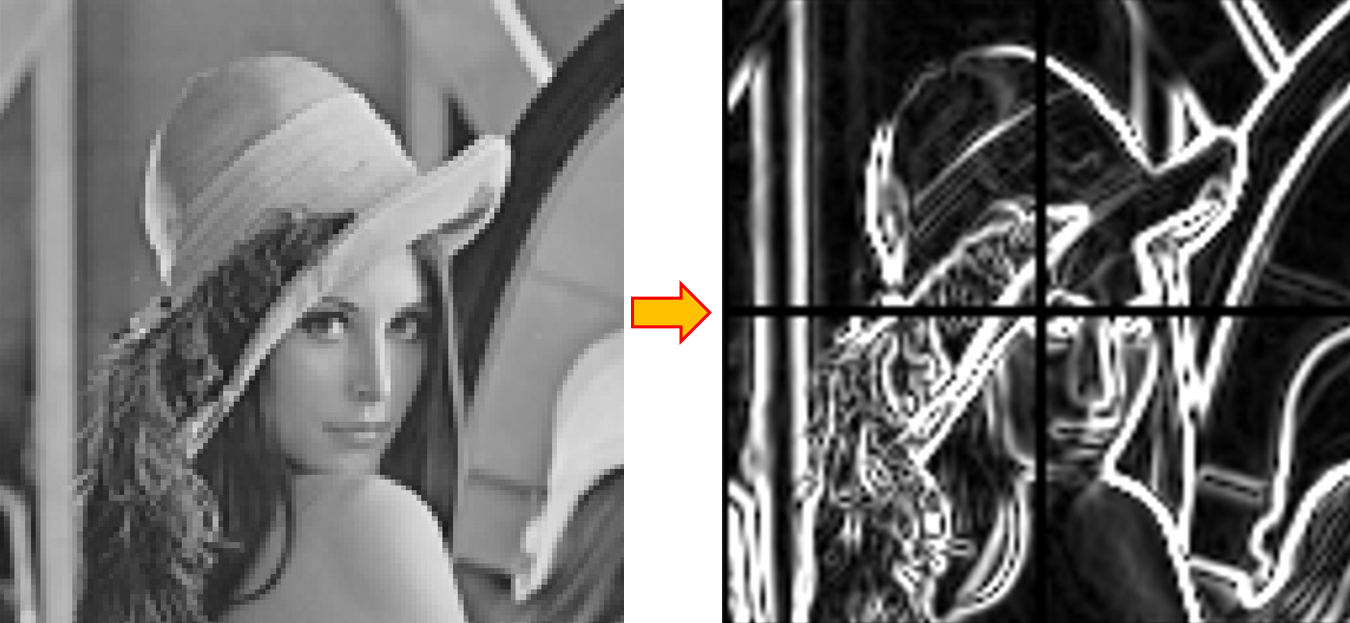
\includegraphics[width=1.0\columnwidth]{img2.png}
    \caption{Avant et après le traitement de l’image}
    \label{fig:5}
\end{figure}

\subsubsection{Temps de traitement}

Le temps nécessaire au système pour traiter les images par les deux Microblazes, après que chaque quart d'entre elles soit placé dans la mémoire partagée, est de 27 ms.

\begin{figure}[H]
    \centering
    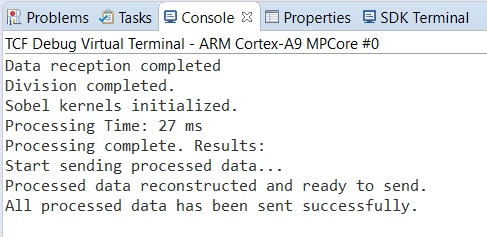
\includegraphics[width=0.5\columnwidth]{./images/Resutlado.jpg}
    \caption{Temps de traitement des images.}
    \label{fig:10}
\end{figure}



\subsection{Système multi-horloge}


Dans ce système, une configuration d'horloges multiples a été implémentée pour gérer les différentes parties de la conception (Figures \ref{fig:6} et \ref{fig:7}). Cela garantit que des modules spécifiques fonctionnent de manière optimale sous différentes fréquences, obtenant ainsi un équilibre entre performances et fonctionnalités du système.

\begin{figure}[H]
    \centering
    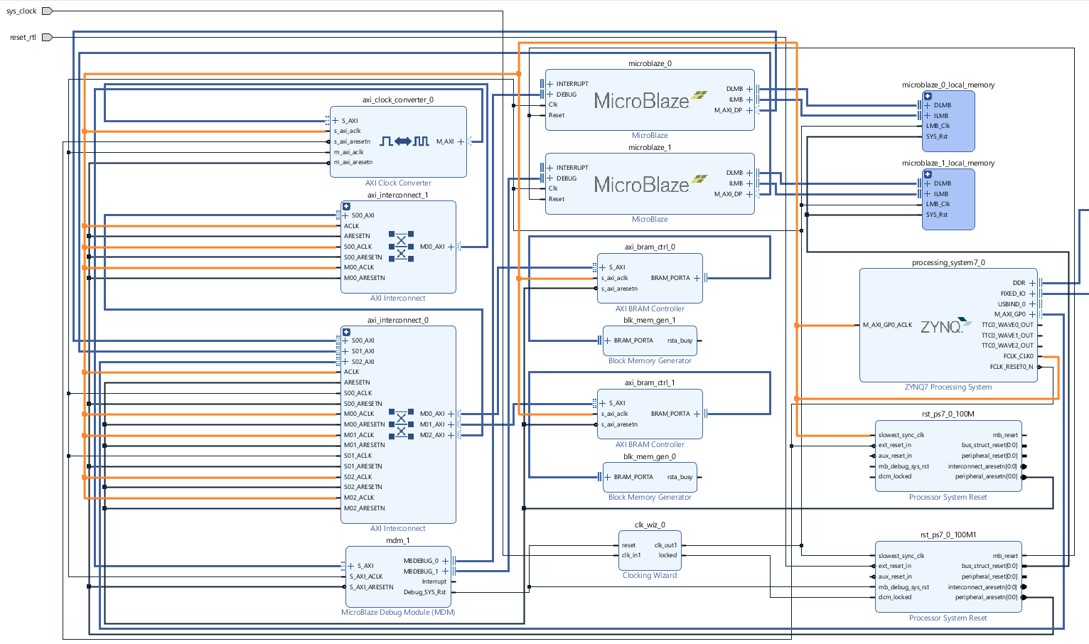
\includegraphics[width=1.0\columnwidth]{./images/MultiReloj1.jpg}
    \caption{Diagramme de blocs: Horloge \# 1}
    \label{fig:6}
\end{figure}



\begin{figure}[H]
    \centering
    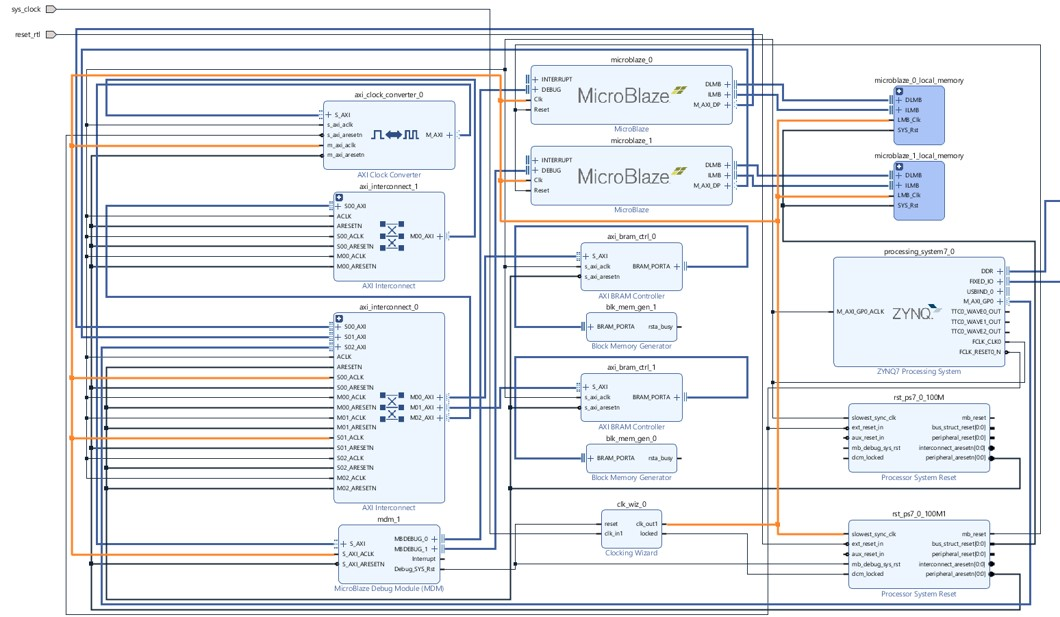
\includegraphics[width=1.0\columnwidth]{./images/MultiReloj2.jpg}
    \caption{Diagramme de blocs: Horloge \# 2}
    \label{fig:7}
\end{figure}


Un \textbf{Clocking Wizard} a été utilisé pour générer et gérer deux fréquences d'horloge différentes dans le système. Ce bloc permet de dériver plusieurs signaux d'horloge à partir d'une source principale, en réglant chacun sur les fréquences souhaitées.
Dans ce cas, l'assistant de pointage a fourni :

\begin{itemize}
    \item Une horloge haute fréquence utilisée pour MicroBlaze, ses mémoires (ILMB, DLMB) et le AXI Memory Mapped Bus (MBA).
    \item Une horloge basse fréquence pour le reste des modules, comme l'ARM 9, la mémoire DDR et les interconnexions AXI.
\end{itemize}

Pour garantir une synchronisation appropriée entre les modules fonctionnant sous différents domaines d'horloge, un \textbf{AXI Clock Converter} a été inclus. Ce bloc facilite la communication entre des périphériques ou des blocs qui fonctionnent avec des fréquences d'horloge différentes au sein d'une interface AXI. Dans cette conception, l'AXI Clock Converter garantissait un transfert de données correct entre le MicroBlaze (avec son domaine d'horloge spécifique) et les modules contrôlés par le ZYNQ.

\vspace{1em} 

Les avantages obtenus avec ce type de configurations sont que chaque module fonctionne à la fréquence qui correspond le mieux à ses besoins fonctionnels, maximisant ainsi l'efficacité sans compromettre la capacité de traitement. De plus, une conception modulaire et efficace est autorisée, adaptée aux besoins spécifiques de chaque composant.
\end{document}
